\documentclass{beamer}

\usepackage[T2A]{fontenc}
\usepackage[utf8]{inputenc}
\usepackage[russian]{babel}
\usepackage{graphicx}
\usepackage{todonotes}

\usetheme{Madrid}
\usecolortheme{whale}

\hypersetup {
    unicode = true
}

\title[]{Инструментальная среда для анализа программных систем}
\author[А.М. Полоцев]{
    А.М. Полоцев, гр. 63501/13\\
    научный руководитель: к.т.н. доцент В.М. Ицыксон
}
\institute[]{Санкт-Петербургский Политехнический Университет}
\date[XLII Неделя науки]{XLII Неделя науки}

\begin{document}
%===============================================================================
\frame{\titlepage}
%===============================================================================
%===============================================================================
\begin{frame}
\frametitle{Постановка задачи}

\begin{itemize}
    \item В различных методах анализа часто решаются похожие задачи:
    \begin{itemize}
        \item Построение моделей программы (AST, CFG и т.п.)
        \item Построение метрик
        \item Реинжиниринг программного обеспечения (оптимизация, рефакторинг и т.п.)
        \item Визуализация свойств системы
    \end{itemize}
\end{itemize}
\pause
\begin{alertblock}{}
    \center{Обычно эти задачи решаются вручную}
\end{alertblock}

\end{frame}
%===============================================================================
%===============================================================================
\begin{frame}
\frametitle{Разработка инструментального средства}

\begin{itemize}
    \item Цели
        \begin{itemize}
            \item Автоматизация анализа
            \item Визуализация свойств системы
        \end{itemize}
    \item Требования
        \begin{itemize}
            \item Поддержка анализа объектно-ориентированных языков
            \item Извлечение различных моделей анализируемой системы
            \item Встроенные средства отображения
            \item Модульная расширяемая структура
            \item Экспорт разных артефактов системы во внешние отчеты
            \item Предоставление API к разработанным методам анализа
        \end{itemize}
\end{itemize}
\end{frame}
%===============================================================================
%===============================================================================
\begin{frame}
\frametitle{Архитектура инструментального средства}

\begin{figure}[h!]
    \begin{center}
        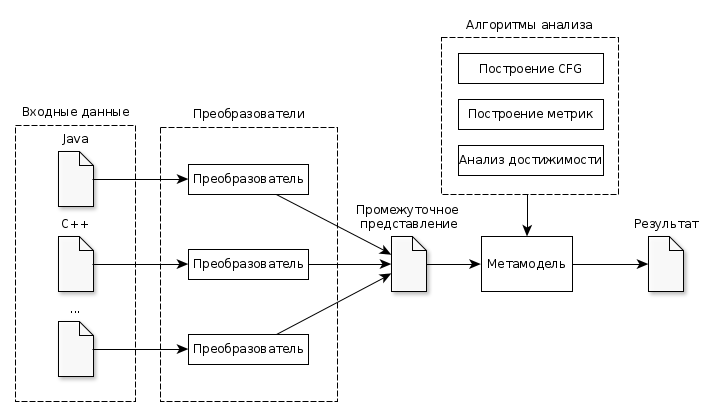
\includegraphics[width=\textwidth]{img/architecture.png}
    \end{center}
\end{figure}
\end{frame}
%===============================================================================
%===============================================================================
\begin{frame}
\frametitle{Разработка метамодели}

\begin{itemize}
    \item Цели:
        \begin{itemize}
            \item Унификация представления системы для проведения анализа и трансформаций
        \end{itemize}
    \item Требования:
        \begin{itemize}
            \item Независимость от языка описания анализируемой системы
            \item Достаточная мощность для извлечения различных моделей
            \item Расширяемость путем добавления новых метаданных
        \end{itemize}
\end{itemize}

\end{frame}
%===============================================================================
%===============================================================================
\begin{frame}
\frametitle{Meta Object Facility (MOF)}

\begin{itemize}
    \item Стандарт, разработанный Object Management Group (OMG)
    \item Метаметамодель для описания метамоделей
    \item Поддержка объектно-ориентированной парадигмы
    \item Четырехуровневая архитектура
    \begin{itemize}
        \item Уровень метаметамодели (M3)
        \item Уровень метамоделей (M2)
        \item Уровень моделей (M1)
        \item Информационный уровень(M0)
    \end{itemize}
\end{itemize}

\end{frame}
%===============================================================================
%===============================================================================
\begin{frame}
\frametitle{Meta Object Facility (MOF)}

\begin{figure}[h!]
    \begin{center}
        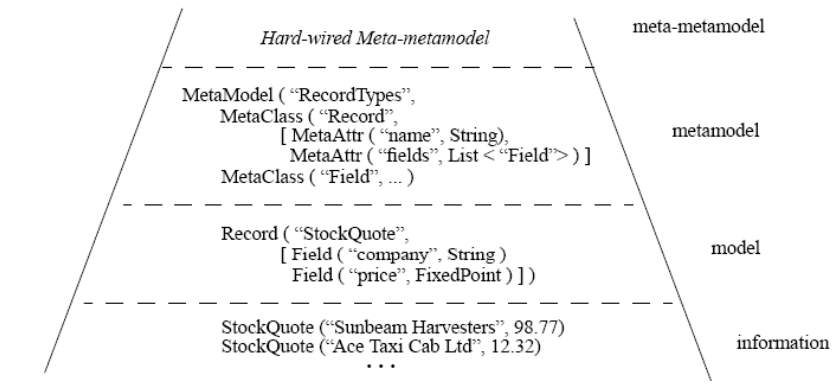
\includegraphics[width=\textwidth]{img/metadata_architecture}
    \end{center}
\end{figure}

\end{frame}
%===============================================================================
%===============================================================================
\begin{frame}
\frametitle{Разработка метамодели}

\missingfigure{Диаграмма классов}

\end{frame}
%===============================================================================
%===============================================================================
\begin{frame}
\frametitle{Преобразование исходного кода в метамодель}

\begin{itemize}
    \item
\end{itemize}

\end{frame}
%===============================================================================
%===============================================================================
\begin{frame}
\frametitle{Спасибо за внимание}
\center{\resizebox{60pt}{80pt}{?}}
\end{frame}
%===============================================================================
\end{document}
